In Chapter~\ref{ch:pes-statistics}, we saw that the photoemission statistics are influenced by the characteristics of the light source, that exhibit well-defined statistical properties. However, when using multidimensional detection schemes capturing millions of voxels, the complexity of the process renders the process difficult to model. Furthermore, the predictive power of such model would rely on an existing understanding the materials, the very aspect under investigation. While the physical process is intriguing to study from a physical perspective, it is not practical for the purpose of image restoration.

Instead of using explicit models such as \gls{BM3D} that encode prior knowledge about the data corruption (e.g. \gls{AWGN}, or Poisson noise as discussed in \cref{sec:poisson-noise-model}), it is also possible to learn the underlying model based on the data. This approach of not hard coding knowledge, and learning complex mappings based on data is the foundation of machine and deep learning, allowing to extract meaningful information from incomplete measurements.

Learning can be broadly categorized in two categories: the \textit{supervised} and the \textit{unsupervised} setting. In supervised learning, the experience (\textit{model}) is learned by exposure to data containing information additional (labeled data) to what the model is supposed to map. The exposure to such data, called \textit{training}, enables the model to establish a relationship between the inputs and their corresponding outputs. The model’s expertise can then be used to map new inputs to their corresponding outputs. In the context of image restoration, the model can gain expertise from pairs of corrupted and clean images, and then use this expertise to restore other corrupted images.

Conversely, in the unsupervised setting, the model is exposed to the data without any labeled information, and the model is supposed to learn the underlying structure of the data. In context of image restoration, that would imply only giving the model the corrupted images, and expecting to map to the desired target--the clean image.

This chapter, we will discuss the foundations of learning, covering the elements of how and why learning works. This is general to both the supervised and unsupervised setting. There the concepts of \textit{hypothesis class}, \textit{capacity}, \textit{realizability}, and the concept of \textit{generalization} capability are discussed. Then we take a look at a statistical learning\footnote{Machine learning and statistical learning are many times used interchangeably but the latter places more emphasis on the statistical properties of the learning algorithms.} paradigm known as \textit{\gls{ERM}}, aiming to minimize the training error/empirical risk. \Gls{ERM} comes with its own set of challenges, such as overfitting in hypothesis spaces with high \textit{capacity}, which can be mitigated by \textit{regularization}. 

We discuss the combination of \textit{\gls{CNN}} and \textit{Autoencoders}, commonly used in image restoration tasks. Later, \textit{Noise2Noise}, a learning framework for image restoration not requiring clean images, introduced by \citeauthor{lehtinenNoise2NoiseLearningImage2018}, is discussed. To fully explain this framework, we look at the \textit{loss function} that allows this paradigm to work. We use the concrete realization using the \texttt{UNET} architecture, introduced \citeauthor{ronnebergerUNetConvolutionalNetworks}, and its 3D variant, \texttt{UNET3D}.

These methods are then applied to train a model that maps incomplete observations from \gls{PES} to the true multidimensional image, with $N=3$. The aspects of data generation, training, and evaluation are henceforth, discussed in detail.

Much of the foundational concepts discussed are based on \cite{shalev-shwartzUnderstandingMachineLearning2014a,jamesIntroductionStatisticalLearning2013,tibshiraniElementsStatisticalLearning,goodfellowDeepLearning2016}.

\section{Foundations of Learning}
Statistical regression is a classical example of a learning algorithm, where the goal of regression is to learn a function that maps the input data to the output data.
Let us approach the image restoration problem from this perspective. Using the general observation model defined in \cref{eq:observation-model}, the learning problem is then to find a hypothesis $h$ that maps the degraded image $X$ to the true image $Y$ that generalizes well.

\begin{equation}
    h: X \mapsto Y
\end{equation}

In Machine Learning, we do not make any explicit assumption of the \textit{data generating distribution} except that all instances of the data are \textit{\gls{iid}} and generated according to a distribution $\mathcal{D}$ i.e. $Y, X \sim \mathcal{D}$.

\subsection{Generalization}
\textit{Generalization} refers to the ability of a learning algorithm to perform well on new, unseen data. The goal of learning is to find a hypothesis $h$ that generalizes well to new data. 

If the data generating distribution $\mathcal{D}$ is \gls{iid} and known, the \textit{generalization error}/\textit{population risk} $\mathcal{R}(\theta)$ with model parameters $\theta$ can be minimized to find the optimal hypothesis $\hat{h}^*$. This is often the case in classical regression 

$\mathcal{R}(\theta)$ is defined as expectation taken across the data generating distribution $\mathcal{D}$, with the predicted output of a hypothesis $h(x; \theta)$ and the true output $y$:

\begin{equation}
    \mathcal{R}(\theta) = \mathbb{E}_{(x, y) \sim \mathcal{D}} \left[ \ell(h(x; \theta), y) \right]
\end{equation}

where the loss $\ell$ measures the difference between two quantities, such as of $h(x; \theta)$ and $y$.

Through optimization, the optimal hypothesis $\hat{h}^*$ can be found that minimizes the expected risk $\mathcal{R}$:

\begin{equation}
    \hat{h}^* = \argmin_{h \in \mathcal{H}} \mathcal{R}(\mathcal{D}; \theta)
\end{equation}

\subsection{Hypothesis Class, Capacity and Realizability}
The hypothesis $h$ is chosen from a hypothesis space $\mathcal{H}$, where the hypothesis space $\mathcal{H}$ is the set of functions that the learning algorithm can choose from to approximate the true function. 
For example, in linear regression, the hypothesis space $\mathcal{H}$ consists of all possible linear functions of the form:

\begin{equation*}
   \mathcal{H} =  \left\{ h_{\mathbf{w}}(\mathbf{x}) = \mathbf{w}^\top \mathbf{x} + w_0 \mid \mathbf{w} \in \mathbb{R}^d, w_0 \in \mathbb{R} \right\}
\end{equation*}

The \textit{capacity} (the measure of size\footnote{The VC dimension and Rademacher complexity are two popular measures of capacity.}) of this hypothesis space is smaller than other hypothesis spaces such as generalized linear models
\footnote{These are linear models with a non-linear activation function, such as sigmoid function.} 
or polynomial class of functions. Choosing a hypothesis class with a larger capacity allows for more complex functions to be learned, but we will see that this comes with a trade-off.

We want to find a space that makes our learning problem \textit{realizable}. This means that there exists a mapping in the hypothesis space that can perfectly model the true mapping. A counter example could be if our data generation function is a $sin(x)$ function, but we choose a linear hypothesis space, then our problem is not realizable. In most real-world scenarios, the true space for complex data such as images is seldom known, and we forego the realizability condition. This is the \textit{agnostic} learning setting. For classes with high capacity, even if they can not perfectly model the true function, they might approximate it well.

\subsection{Empirical Risk Minimization}

In the case where true data distribution $\mathcal{D}$ is unknown, and the learning algorithm must make predictions on new data that sampled from $\mathcal{D}$.
The most popular learning algorithm is known as \textit{\glsxtrlong{ERM}}. For a training set $\mathcal{S} = \left\{ (x_1, y_1), \ldots, (x_n, y_n) \right\}$ where $\mathcal{S} \sim \mathcal{D}^n$, and model parameters $\theta$, the empirical risk $\mathcal{L}(\theta; \mathcal{S})$ is defined as:

\begin{equation}
    \mathcal{L}(\mathcal{S}; \theta) = \frac{1}{\lvert \mathcal{S} \rvert} \sum_{(x, y) \in \mathcal{S}} \ell(h(x; \theta), y),
\end{equation}

where $\ell$ is the loss function that measures the error between the predicted output $h(x; \theta)$ and the true output $y$ mapped from $\mathcal{G} (x)$. The \gls{ERM} algorithm finds the hypothesis $\hat{h}$ from hypothesis space $\mathcal{H}$ that minimizes the training error $\mathcal{L}$

\begin{equation}
    \hat{h} = \argmin_{h \in \mathcal{H}} \mathcal{L}(\theta; \mathcal{S})
\end{equation}

We shall later see that the assumption of output  $y = \mathcal{G} (x)$ can be relaxed in the \textit{Noise2Noise} framework with an \gls{MSE} $\ell$.

\subsection{Regularization}
The \gls{ERM} algorithm runs the risk of \textit{overfitting}. This means that the hypothesis $\hat{h}$ might perform well on the training data $\mathcal{S}$ but poorly on new data drawn from the same distribution $\mathcal{D}$. Usually, this happens for rich hypothesis classes (high capacity), or $\mathcal{S}$ is not representative of $\mathcal{D}$ and the \gls{ERM} algorithm chooses a hypothesis that is too complex. 

To counter this, \textit{regularization} techniques are used. A penalty term based on model parameters is added to prevent overfitting. The \gls{ERM} then finds the hypothesis $\hat{h}$ that minimizes the regularized loss function\footnote{This is also known as Regularizated Loss Minimization (RLM)}:

\begin{equation}
    \hat{h} = \argmin_{h \in \mathcal{H}} \left(\mathcal{L}(\theta; \mathcal{S})  + \lambda R(\theta) \right).
\end{equation}

where $R(\theta)$ is the regularization term that penalizes complex models, and $\lambda$ is the parameter controlling the trade-off between the training error and the regularization term. Common regularization techniques include L1 (Lasso) and L2 (Ridge) regularization. L1 regularization can be written as:

\begin{equation*}
    R(\theta) = \|\theta\|_1 = \sum{j} |\theta_j|
\end{equation*}

and L2 regularization as:

\begin{equation*}
    R(\theta) = \|\theta\|^2_2 = \sum_{j} \theta_j^2
\end{equation*}

Regularization can also be seen as a way of restricting the hypothesis space $\mathcal{H}$ by encoding prior knowledge into the model. In the case of image restoration, it might be known a priori that the image is smooth, and  can encode this prior knowledge by adding a penalty term that penalizes sharp changes in the image.


\subsection{Uniform Convergence}
It is always possible that with a small probability, the training data is not representative of the data distribution $\mathcal{D}$. Hence, every learning algorithm has a confidence and accuracy level that, in practice, is hard to quantify. For simpler cases, these bounds can be theoretically proven but practically, other evaluation methods are assumed e.g. by empirically evaluating some test data, we can ascertain the if the learned model generalizes well.

For a hypothesis space $\mathcal{H}$ that is finite, and \gls{iid} training data all drawn from the same distribution $\mathcal{D}$, the \gls{ERM} algorithm can be shown to have a generalization error that converges to zero as the number of training samples $n$ goes to infinity. This is known as the \textit{uniform convergence} property of the \gls{ERM} algorithm. This can further be generalized to infinite hypothesis spaces.


The finite hypothesis space assumption makes sense, considering that we learn through discrete data, and infinite hypothesis spaces become finite. 


\section{Noise2Noise: Deep Learning framework}
One can do a lot of different learning approaches. We will build towards the deep learning approach. Networks which can deal with image data are generally Convolutional Neural Networks. Looking at research, UNET has been used for image segmentation and denoising, which combines the concept of autoencoders and convolutional neural networks, along with skip connections.
We use this approach with the noise2noise framework, which is a deep learning framework for image reconstruction.

For classical learning algorithms, the learning problem is not always realizable, meaning that not always is the 
ERM 
Linear separators are restrictive
Deep learning is just linear sepeartor problem with a non linear function applied to it like RELU



Important to take care not to train with empty data. \cite{lehtinenNoise2NoiseLearningImage2018}

Here we take care of data generation. Finite Capture Budget. We use the Graphene on Iridium dataset. The Noisy realizations are just less counts binned. 
E.g. 96M counts as Noisy and 186M counts as Target. Or 8M counts as Noisy and 96M counts as Target.
\subsection{Convolutional Neural Networks}
\subsection{Autoencoder}
\cite{goodfellowDeepLearning2016}
\subsection{UNET}


The benefits of 3D network can be explained by access to more correlations in the data. maybe blessing of dimensionality.

\section{Training}

\begin{figure}[h]
    \centering
    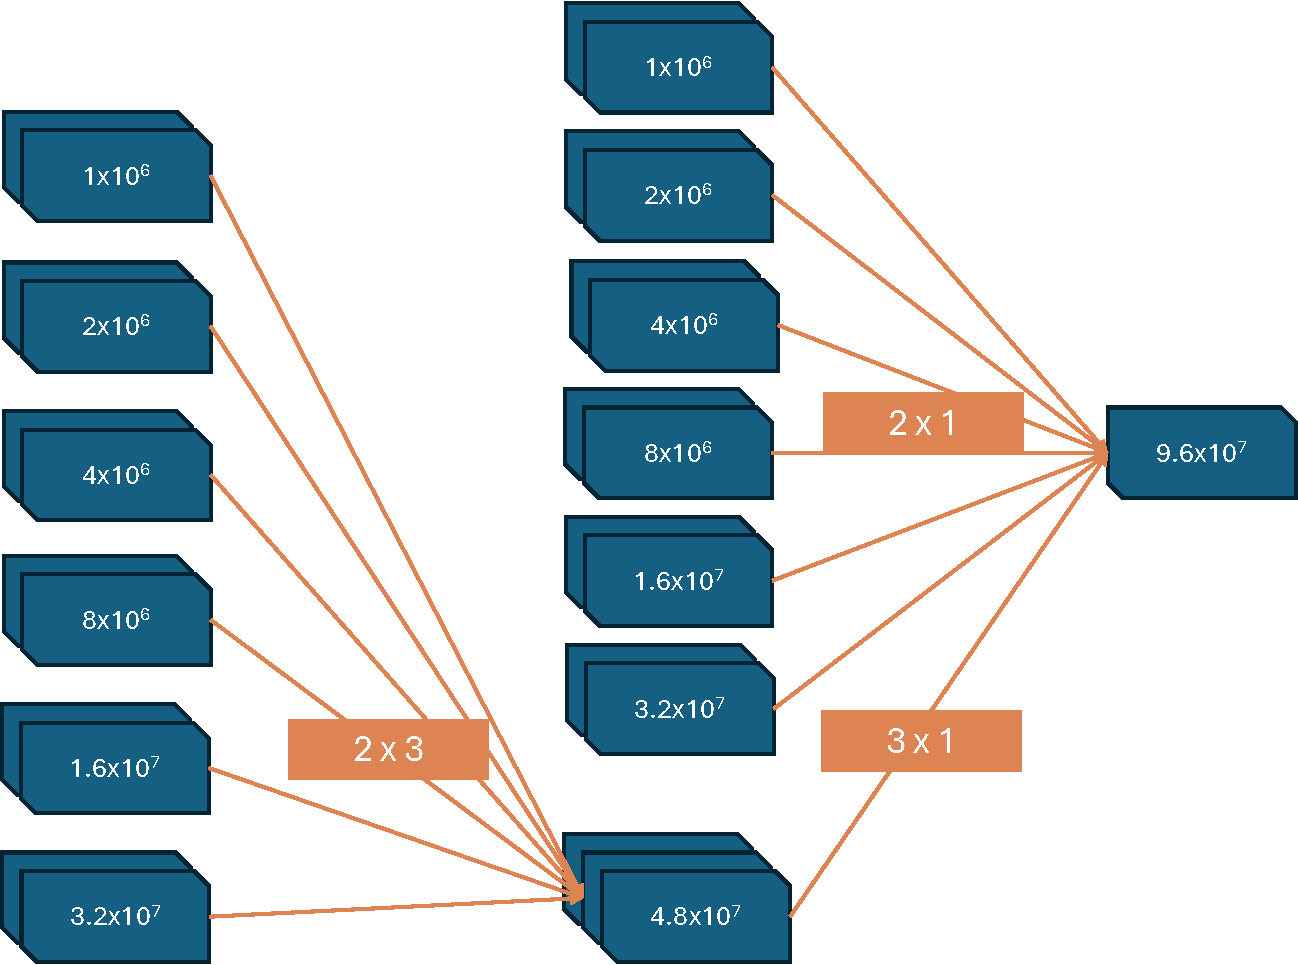
\includegraphics[width=1\linewidth]{images/training_flowchart.pdf}
    \caption{Flowchart illustrating the input-target dataset pairs used for neural network training, derived from subsets of the \gls{GrIr} dataset. A total of \num{34} unique noisy subsets are represented, with each dataset corresponding to one blue box in the chart. The different combinations shown in the chart generate \num{51} input-target pairs across various counts, including \numlist{1e6;2e6;4e6;8e6;1.6e7;3.2e7;4.8e7;9.6e7}. Notably, the \num{4.8e7} and \num{9.6e7} counts serve as the target datasets, with \num{9.6e7} additionally functioning as the target for the \num{4.8e7} datasets.}
    \label{fig:training-data}
\end{figure}